\title{ A Traveling Salesman Solution For The Capitals of All African Nations }
\author{
Brian Gianforcaro \\
Department of Computer Science\\
Rochester Institute of Technology\\
}

\date{\today}

\documentclass[12pt]{article}

\usepackage{graphicx}
\usepackage{multicol}
\usepackage{mdwlist}
\usepackage{amssymb,amsmath}
\usepackage{cite}
\usepackage[bookmarks=false,colorlinks=true,linkcolor={blue},pdfstartview={XYZ null null 1.22}]{hyperref}
\usepackage{url}
\usepackage[T1]{fontenc}
%\usepackage{gfsartemisia-euler}


\begin{document}
\maketitle

\begin{abstract}
  A Traveling Salesman Problem is the task of finding
the shortest round trip path a traveling salesperson can take
to visit each vertex of a given graph.  They are usually
implemented using a genetic algorithm. Our salesperson
happens to be traveling to the capitals of every country in Africa that is a recognized member of the United Nations.
\end{abstract}

\section{The Problem}

  Attempt to find the shorest i.e. cheapest complete path around all African Nations so our sales person can travel the most efficient route possible.

\begin{figure}[h!]
  \begin{center}
    \setlength\fboxsep{1.00pt}
    \setlength\fboxrule{1.00pt}
    \fbox{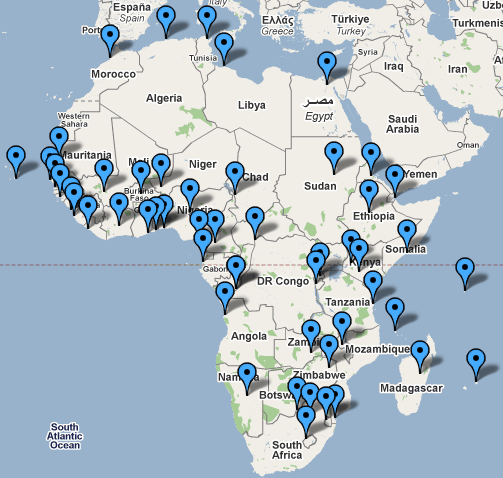
\includegraphics[scale=0.60]{points.png}}
    \caption{Capitals of African Nations}
  \end{center}
\end{figure}


\begin{multicols}{3}
\tiny\begin{enumerate*}
\item Algeria - Algiers
\item Angola - Luanda
\item Benin - Porto-Novo
\item Botswana - Gaborone
\item Burkina Faso - Ouagadougou
\item Burundi - Bujumbura
\item Cameroon - Yaounde
\item Cape Verde - Praia
\item Central African Republic - Bangui
\item Chad - N'Djamena
\item Comoros - Moroni
\item Congo, Republic of the - Brazzaville
\item Congo, Democratic Republic of the - Kinshasa
\item Cote d'Ivoire - Yamoussoukro
\item Djibouti - Djibouti
\item Egypt - Cairo
\item Equatorial Guinea - Malabo
\item Eritrea - Asmara
\item Ethiopia - Addis Ababa
\item Gabon - Libreville
\item The Gambia - Banjul
\item Ghana - Accra
\item Guinea - Conakry
\item Guinea-Bissau - Bissau
\item Kenya - Nairobi
\item Lesotho - Maseru
\item Liberia - Monrovia
\item Libya - Tripoli
\item Madagascar - Antananarivo
\item Malawi - Lilongwe
\item Mali - Bamako
\item Mauritania - Nouakchott
\item Mauritius - Port Louis
\item Morocco - Rabat
\item Mozambique - Maputo
\item Namibia - Windhoek
\item Niger - Niamey
\item Nigeria - Abuja
\item Rwanda - Kigali
\item Senegal - Dakar
\item Seychelles - Victoria
\item Sierra Leone - Freetown
\item Somalia - Mogadishu
\item South Africa - Pretoria
\item Sudan - Khartoum
\item Swaziland - Mbabane
\item Tanzania - Dar es Salaam
\item Togo - Lome
\item Tunisia - Tunis
\item Uganda - Kampala
\item Zambia - Lusaka
\item Zimbabwe - Harare
\end{enumerate*}
\end{multicols}

\section{Overview}

  The traveling salesman problem (TSP) is a thoroughly researched problem in theoreticaly computer-science. 
TSP is classified as NP-Hard eg. as hard or harder to solve than a problem solvable in nondeterministic polynomial time.
This means the worst case performance for a TSP algorithm will likely increase exponetially with the numbers of cities to traverse.
The big-O complexity of a brute force TSP algorithms (check all vertices against all other vertices) is $O(n!)$.

\section{Programs}

\begin{enumerate}
\item The Python 2.6 \cite{python} programming language and interpreter.
\item Wikipedia's list of city latitude/longitudes \cite{wiki}.
\item Software originally written by John Montgomery \cite{tsp} in 2007.General exercise in different types of TSP solving algorithms.
\item The results were then visualized using Google maps static mapping API \cite{google}.

\end{enumerate}


\section{Solution}

%$yDis = ( lat2 - lat1 ) * \text{Nautical Miles Per Latitude}$\newline
%$xDis = ( \cos( lat1 - \frac{\pi}{180} ) + \cos( lat2 - \frac{\pi}{180} ) ) * ( lon2 - lon1 ) * \frac{\text{Nautical Miles Per Longitude}}{2}$\newline
%$tDistance = \sqrt{ yDis^{2} + xDis^{2} } * \text{Miles per Nautical Miles}$\newline


\begin{figure}[!h]
  \begin{center}
    \setlength\fboxsep{1.00pt}
    \setlength\fboxrule{1.00pt}
    \fbox{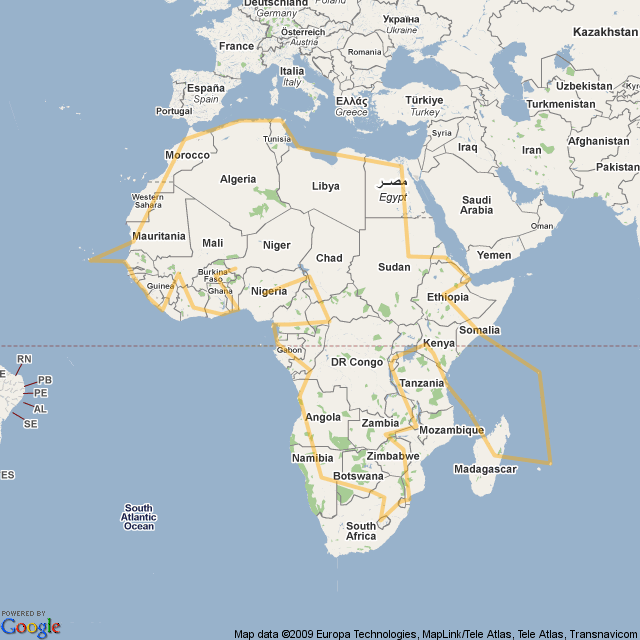
\includegraphics[scale=0.50]{path.png}}
    \caption{Final Path Through Africa}
  \end{center}
\end{figure}

Final Order:
\begin{multicols}{3}
\tiny\begin{enumerate*}
\item Congo, Republic of the - Brazzaville
\item Congo, Democratic Republic of the - Kinshasa
\item Angola - Luanda
\item Namibia - Windhoek
\item Botswana - Gaborone
\item South Africa - Pretoria
\item Lesotho - Maseru
\item Swaziland - Mbabane
\item Mozambique - Maputo
\item Zimbabwe - Harare
\item Zambia - Lusaka
\item Malawi - Lilongwe
\item Burundi - Bujumbura
\item Rwanda - Kigali
\item Uganda - Kampala
\item Kenya - Nairobi
\item Tanzania - Dar es Salaam
\item Comoros - Moroni
\item Madagascar - Antananarivo
\item Mauritius - Port Louis
\item Seychelles - Victoria
\item Somalia - Mogadishu
\item Ethiopia - Addis Ababa
\item Djibouti - Djibouti
\item Eritrea - Asmara
\item Sudan - Khartoum
\item Egypt - Cairo
\item Libya - Tripoli
\item Tunisia - Tunis
\item Algeria - Algiers
\item Morocco - Rabat
\item Mauritania - Nouakchott
\item Cape Verde - Praia
\item Senegal - Dakar
\item The Gambia - Banjul
\item Guinea-Bissau - Bissau
\item Guinea - Conakry
\item Sierra Leone - Freetown
\item Liberia - Monrovia
\item Cote d'Ivoire - Yamoussoukro
\item Mali - Bamako
\item Burkina Faso - Ouagadougou
\item Niger - Niamey
\item Ghana - Accra
\item Togo - Lome
\item Benin - Porto-Novo
\item Nigeria - Abuja
\item Chad - N'Djamena
\item Central African Republic - Bangui
\item Cameroon - Yaounde
\item Equatorial Guinea - Malabo
\item Gabon - Libreville
\end{enumerate*}
\end{multicols}

Total Round Trip $\approx 22253.2035387$ miles

\section{Runtime}

The two algorithms, simulated annealing and brute force random permutations where both run in numerious instances over the life of the project. 
In combined total they were run upwards of fity times a peice.

The version of the algorithm wich used simulated annealing on average found the optimal solution in 6 seconds. 
While the bruteforce method often took upwards of 

\section{Analysis}

I believe the final optimal path's are within a reasonable uncertenty of the actual path.
Given the big-O of the brute force algorithm $O(n!)$ or $O(80658175170943878571660636856403766975289505440883277824000000000000)$ a runtime complexity of this magnitude is obviously out of my leauge for finding exact values.
At a maxiumum I was able to attempt 100,000,000 permutations of the path.

Two area's of possible improvement I can pinpoint are:
\begin{enumerate}
\item The language itself. I chose the python programming language for my TSP implementation.
The language is interpreted and it's runtime speed can at times be 20\% slower than an equivilant C program.
\item The random.shuffle implementation. Given how python's random.shuffle API is implemented it talkes a set
of values and shuffles them based on a random number between 0,1 generated by the operating system. However given the size of the set
, 52 individual points, the likely hood that random.shuffle will generated all permutations without excessive doubles is increadibly unlikely.
This is the cause of a lot of literally useless computation time, however because of the size of the data set, caching data sets is not plausible let alone if even possible.
\end{enumerate}

Re-writing the algorithm in C would be a great performance benifit. Also having a proper resources to cache routes or a effective random route generater I beleive a more accurate optimal route might be found.

\begin{thebibliography}{99}
\bibitem{python} {\href{ http://python.org }{ http://python.org }}
\bibitem{wiki} {\href{ http://en.wikipedia.org/wiki/Latitude_and_longitude_of_cities }{ http://en.wikipedia.org/wiki/Latitude\_and\_longitude\_of\_cities }}
\bibitem{tsp} Montgomery, John {\it Tackling The Travelling Salesman Problem }{\href{ http://www.psychicorigami.com/category/tsp/ }{ http://www.psychicorigami.com/category/tsp/ } }, {\bf 2007}
\bibitem{google} {\href{ http://code.google.com/apis/maps/documentation/staticmaps/  }{ http://code.google.com/apis/maps/documentation/staticmaps/ }}

\end{thebibliography}
\end{document}
